\documentclass[tikz,border=5pt]{standalone}
\usepackage[T1]{fontenc}
\usepackage{lmodern}
\usepackage{pgfplots}
\usepgfplotslibrary{groupplots}
\usetikzlibrary{shapes.geometric}
\pgfplotsset{compat=1.18}
\definecolor{runone}{RGB}{110,110,110}
\definecolor{runtwo}{RGB}{38,108,165}
\definecolor{runthree}{RGB}{211,122,42}
% Generated by scripts/build_three_run_evidence.py from private aggregate evidence.
\def\RunOneLabel{Run 1}
\def\RunOneArtifacts{365}
\def\RunOneProvenance{365}
\def\RunTwoLabel{Run 2}
\def\RunTwoArtifacts{365}
\def\RunTwoProvenance{365}
\def\RunThreeLabel{Run 3}
\def\RunThreeArtifacts{365}
\def\RunThreeProvenance{365}
\def\RopBinLabels{{3--29},{29--221},{0.2k--1.7k},{1.7k--12.3k},{12.3k--91.7k},{91.7k--683.0k}}
\def\RopAxisTicks{1,2,3,4,5,6}
\def\RopAxisTickLabels{{1},{2},{3},{4},{5},{6}}
\def\RopBinKey{1: 3--29\quad 2: 29--221\quad 3: 0.2k--1.7k\quad 4: 1.7k--12.3k\quad 5: 12.3k--91.7k\quad 6: 91.7k--683.0k}
\def\RopRunOneHistogram{(1,3) (2,21) (3,162) (4,126) (5,42) (6,11)}
\def\RopRunTwoHistogram{(1,4) (2,21) (3,161) (4,130) (5,37) (6,12)}
\def\RopRunThreeHistogram{(1,3) (2,22) (3,172) (4,116) (5,40) (6,12)}
\def\OqBinLabels{{63--302},{0.3k--1.4k},{1.4k--6.8k},{6.8k--32.2k},{32.2k--152.4k},{152.4k--721.8k}}
\def\OqAxisTicks{1,2,3,4,5,6}
\def\OqAxisTickLabels{{1},{2},{3},{4},{5},{6}}
\def\OqBinKey{1: 63--302\quad 2: 0.3k--1.4k\quad 3: 1.4k--6.8k\quad 4: 6.8k--32.2k\quad 5: 32.2k--152.4k\quad 6: 152.4k--721.8k}
\def\OqRunOneHistogram{(1,14) (2,83) (3,164) (4,62) (5,30) (6,12)}
\def\OqRunTwoHistogram{(1,15) (2,82) (3,164) (4,63) (5,29) (6,12)}
\def\OqRunThreeHistogram{(1,16) (2,81) (3,164) (4,62) (5,30) (6,12)}
\def\SsBinLabels{{0--7},{7--65},{65--536},{0.5k--4.4k},{4.4k--35.5k},{35.5k--288.7k}}
\def\SsAxisTicks{1,2,3,4,5,6}
\def\SsAxisTickLabels{{1},{2},{3},{4},{5},{6}}
\def\SsBinKey{1: 0--7\quad 2: 7--65\quad 3: 65--536\quad 4: 0.5k--4.4k\quad 5: 4.4k--35.5k\quad 6: 35.5k--288.7k}
\def\SsRunOneHistogram{(1,4) (2,10) (3,130) (4,165) (5,43) (6,13)}
\def\SsRunTwoHistogram{(1,3) (2,11) (3,132) (4,163) (5,42) (6,14)}
\def\SsRunThreeHistogram{(1,5) (2,11) (3,129) (4,164) (5,43) (6,13)}
\def\FigureThreeFootnote{All values use the shared material cohort (n=365). Runs 2--3: 365 provenance-matched policy pairs; 36 exact numeric triples.}


\begin{document}
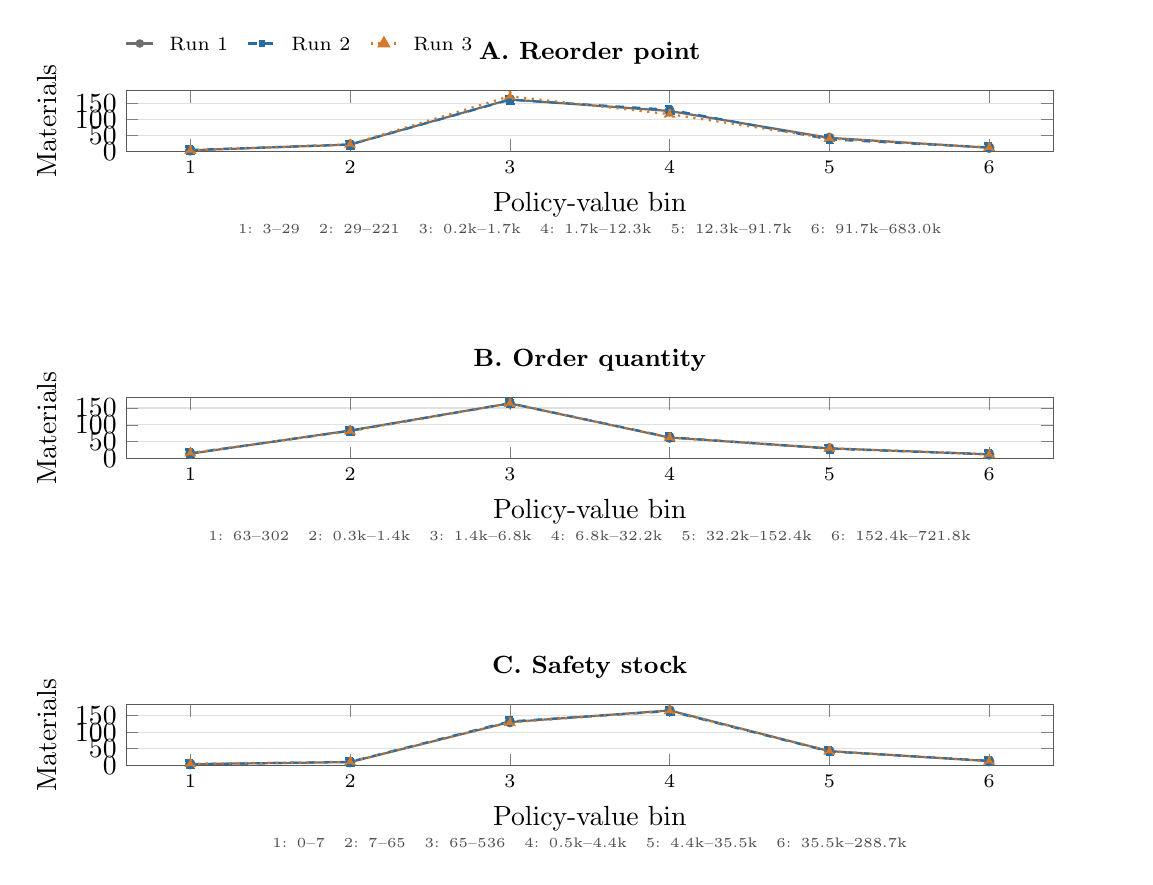
\begin{tikzpicture}
\draw[runone,thick] (0,0) -- +(0.34,0) node[pos=0.5,circle,fill=runone,inner sep=1.1pt]{};
\node[anchor=west,font=\scriptsize] at (0.42,0) {Run 1};
\draw[runtwo,thick,dashed] (1.55,0) -- +(0.34,0) node[pos=0.5,rectangle,fill=runtwo,inner sep=1.1pt]{};
\node[anchor=west,font=\scriptsize] at (1.97,0) {Run 2};
\draw[runthree,thick,dotted] (3.10,0) -- +(0.34,0) node[pos=0.5,regular polygon,regular polygon sides=3,fill=runthree,inner sep=1.0pt]{};
\node[anchor=west,font=\scriptsize] at (3.52,0) {Run 3};
\begin{scope}[yshift=-0.6cm]
\begin{axis}[
  name=ropaxis,
  at={(0,0)},anchor=north west,
  width=13.35cm,height=2.35cm,
  ymin=0,ymajorgrids=true,
  grid style={black!12},
  axis line style={black!65},
  xlabel={Policy-value bin},
  ylabel={Materials},
  xtick/.expand once=\RopAxisTicks,
  xticklabels/.expand once=\RopAxisTickLabels,
  xticklabel style={font=\scriptsize},
  title style={font=\small\bfseries},
  title={A. Reorder point},
  enlarge x limits=0.08,
]
  \addplot[runone,thick,mark=*,mark size=1.5pt,mark options={fill=runone,draw=none}] coordinates {\RopRunOneHistogram};
  \addplot[runtwo,thick,dashed,mark=square*,mark size=1.4pt,mark options={fill=runtwo,draw=none}] coordinates {\RopRunTwoHistogram};
  \addplot[runthree,thick,dotted,mark=triangle*,mark size=1.7pt,mark options={fill=runthree,draw=none}] coordinates {\RopRunThreeHistogram};
\end{axis}
\node[anchor=north,font=\tiny,text=black!70,text width=13.35cm,align=center] at ([yshift=-0.8cm]ropaxis.south) {\RopBinKey};
\end{scope}
\begin{scope}[yshift=-4.5cm]
\begin{axis}[
  name=oqaxis,
  at={(0,0)},anchor=north west,
  width=13.35cm,height=2.35cm,
  ymin=0,ymajorgrids=true,
  grid style={black!12},
  axis line style={black!65},
  xlabel={Policy-value bin},
  ylabel={Materials},
  xtick/.expand once=\OqAxisTicks,
  xticklabels/.expand once=\OqAxisTickLabels,
  xticklabel style={font=\scriptsize},
  title={B. Order quantity},
  title style={font=\small\bfseries},
  enlarge x limits=0.08,
]
  \addplot[runone,thick,mark=*,mark size=1.5pt,mark options={fill=runone,draw=none}] coordinates {\OqRunOneHistogram};
  \addplot[runtwo,thick,dashed,mark=square*,mark size=1.4pt,mark options={fill=runtwo,draw=none}] coordinates {\OqRunTwoHistogram};
  \addplot[runthree,thick,dotted,mark=triangle*,mark size=1.7pt,mark options={fill=runthree,draw=none}] coordinates {\OqRunThreeHistogram};
\end{axis}
\node[anchor=north,font=\tiny,text=black!70,text width=13.35cm,align=center] at ([yshift=-0.8cm]oqaxis.south) {\OqBinKey};
\end{scope}
\begin{scope}[yshift=-8.4cm]
\begin{axis}[
  name=ssaxis,
  at={(0,0)},anchor=north west,
  width=13.35cm,height=2.35cm,
  ymin=0,ymajorgrids=true,
  grid style={black!12},
  axis line style={black!65},
  xlabel={Policy-value bin},
  ylabel={Materials},
  xtick/.expand once=\SsAxisTicks,
  xticklabels/.expand once=\SsAxisTickLabels,
  xticklabel style={font=\scriptsize},
  title={C. Safety stock},
  title style={font=\small\bfseries},
  enlarge x limits=0.08,
]
  \addplot[runone,thick,mark=*,mark size=1.5pt,mark options={fill=runone,draw=none}] coordinates {\SsRunOneHistogram};
  \addplot[runtwo,thick,dashed,mark=square*,mark size=1.4pt,mark options={fill=runtwo,draw=none}] coordinates {\SsRunTwoHistogram};
  \addplot[runthree,thick,dotted,mark=triangle*,mark size=1.7pt,mark options={fill=runthree,draw=none}] coordinates {\SsRunThreeHistogram};
\end{axis}
\node[anchor=north,font=\tiny,text=black!70,text width=13.35cm,align=center] at ([yshift=-0.8cm]ssaxis.south) {\SsBinKey};
\end{scope}
\end{tikzpicture}
\end{document}
